\documentclass[aspectratio=169,10pt]{beamer}

% ---------------------------------------------------------------------------
% Packages
% ---------------------------------------------------------------------------
\usepackage[utf8]{inputenc}
\usepackage[T1]{fontenc}
\usepackage{lmodern}
\usepackage{graphicx}
\usepackage{booktabs}
\usepackage{siunitx}
\usepackage{array}
\usepackage{enumitem}
\usepackage{tikz}
\usepackage{pgfplots}
\pgfplotsset{compat=1.17}
\usetikzlibrary{arrows.meta,positioning,shapes.geometric,calc}
\usepackage{multirow}

\sisetup{table-number-alignment = center}

% ---------------------------------------------------------------------------
% Color palette (navy / blue), same as progress deck
% ---------------------------------------------------------------------------
\definecolor{navy}{RGB}{16,32,63}
\definecolor{steel}{RGB}{43,92,157}
\definecolor{steellight}{RGB}{140,175,214}
\definecolor{bgpanel}{RGB}{240,243,247}
\definecolor{graytext}{RGB}{95,95,95}
\definecolor{municblue}{RGB}{100,140,190}
\definecolor{psuborange}{RGB}{222,164,101}
\definecolor{ppagbrown}{RGB}{150,98,58}
\definecolor{schoolgreen}{RGB}{80,165,130}
\definecolor{neutralgray}{RGB}{176,182,192}
\definecolor{statusred}{RGB}{176,36,36}
\definecolor{statuspink}{RGB}{204,100,100}
\definecolor{statuslisto}{RGB}{40,120,70}
\definecolor{placeholderbg}{RGB}{252,242,230}
\definecolor{placeholderline}{RGB}{196,120,40}

% ---------------------------------------------------------------------------
% Minimalist theme
% ---------------------------------------------------------------------------
\usetheme{default}
\setbeamertemplate{navigation symbols}{}
\setbeamertemplate{headline}{}

\setbeamercolor{normal text}{fg=black,bg=white}
\setbeamercolor{structure}{fg=navy}
\setbeamercolor{title}{fg=white,bg=navy}
\setbeamercolor{frametitle}{fg=navy,bg=white}
\setbeamercolor{alerted text}{fg=steel}
\setbeamercolor{block title}{fg=white,bg=steel}
\setbeamercolor{block body}{fg=black,bg=bgpanel}
\setbeamercolor{itemize item}{fg=steel}
\setbeamercolor{itemize subitem}{fg=steellight}
\setbeamerfont{frametitle}{series=\bfseries}
\setbeamerfont{footline}{size=\scriptsize}

\setbeamertemplate{itemize item}{\raise1.2pt\hbox{\textcolor{steel}{\rule{4pt}{4pt}}}}
\setbeamertemplate{itemize subitem}{\raise1.2pt\hbox{\textcolor{steellight}{\rule{3pt}{3pt}}}}

\setlist[itemize]{itemsep=5pt, topsep=3pt, leftmargin=*}
\setlist[itemize,2]{itemsep=3pt, topsep=2pt}
\setlist[enumerate]{itemsep=5pt, topsep=3pt, leftmargin=*}

\setbeamertemplate{frametitle}{
  \vspace{0pt}
  \hspace{2pt}\textcolor{navy}{\large\bfseries\insertframetitle}\par
  \vspace{-4pt}
  \hspace{2pt}\textcolor{steel}{\rule{0.94\paperwidth}{0.7pt}}
  \vspace{-8pt}
}

\setbeamertemplate{footline}{
  \hfill
  \raisebox{6pt}{\textcolor{graytext}{\scriptsize\insertframenumber\,/\,\inserttotalframenumber}}
  \hspace{10pt}
  \vspace{6pt}
}

\setbeamertemplate{blocks}[rounded][shadow=false]

\newcommand{\fuente}[1]{\vspace{2pt}\textcolor{graytext}{\scriptsize #1}}

% One-line slide conclusion
\newcommand{\takeaway}[1]{\par\vspace{6pt}{\small\textcolor{steel}{$\Rightarrow$}\ \textbf{\textcolor{navy}{#1}}}}

% Placeholder box for pending results
\newcommand{\placeholder}[1]{%
  \begin{tikzpicture}
  \node[draw=placeholderline,thick,dashed,fill=placeholderbg,rounded corners,
        text width=0.85\textwidth,align=center,inner sep=14pt] {%
    \textcolor{placeholderline}{\Large $\varnothing$}\\[6pt]
    \textcolor{placeholderline}{\bfseries PLACEHOLDER --- results pending}\\[4pt]
    \small\textcolor{graytext} #1
  };
  \end{tikzpicture}
}

\title{Impacts of Public Early Childhood Education in Chile on Maternal Fertility and Labor Market Outcomes}
\author{Micaella Magnasco}
\date{October 2026}

\begin{document}

% =============================================================================
% 1. TITLE
% =============================================================================
\begin{frame}[plain]
\vspace{40pt}
\begin{center}
{\LARGE\bfseries\color{navy} Impacts of Public Early Childhood Education\\[3pt] in Chile on Maternal Fertility\\[3pt] and Labor Market Outcomes}

\vspace{8pt}
{\large\color{graytext} Short-run effects --- progress update}

\vspace{10pt}
\textcolor{steel}{\rule{0.5\paperwidth}{0.6pt}}

\vspace{18pt}
{\normalsize
Andr\'es Hojman \quad Marigen Narea \quad Jorge Rodr\'iguez \quad Pedro Carneiro \quad Micaella Magnasco\\[8pt]
\small Pontificia Universidad Cat\'olica de Chile \\[2pt]
\small October 2026
}
\end{center}
\end{frame}

% =============================================================================
% 1b. EXECUTIVE SUMMARY
% =============================================================================
\begin{frame}
\vspace{4pt}
{\large\bfseries\color{navy} Where we are}
\vspace{8pt}

\begin{columns}[T]
\begin{column}{0.49\textwidth}
{\small\textcolor{steel}{\textbf{What we do}}}
\begin{itemize}
  \footnotesize
  \item \textbf{Question}: does opening a public preschool nearby change mothers' labor supply and fertility?
  \item \textbf{Variation}: 447 neighborhood units (UVs) open their \emph{first} JUNJI/Integra preschool in 2015--2024 vs.\ 4{,}145 that never do
  \item \textbf{Design}: staggered event study at the UV level, Sun--Abraham estimator (Baker et al., \emph{JEL} 2026)
  \item \textbf{Data}: woman-level panel linking administrative registries --- RSH/FPS, SII/AFP earnings, Civil Registry births, preschool enrollment
\end{itemize}
\end{column}
\begin{column}{0.49\textwidth}
{\small\textcolor{steel}{\textbf{What we find so far}}}
\begin{itemize}
  \footnotesize
  \item \textbf{Balance}: in 2014, women in treated and never-treated UVs look alike; UVs differ in \emph{size} $\to$ UV + year FE
  \item \textbf{First stage}: enrollment rises $\approx$\textbf{2pp} on a 33\% base ($\approx$6\%) the year a preschool opens, persistent and robust across 3 estimators
  \item \textbf{Labor \& fertility}: estimates in progress
\end{itemize}
\end{column}
\end{columns}

\vspace{10pt}
\begin{block}{Project status}
\footnotesize
\begin{tabular}{@{}>{\raggedright\arraybackslash}p{0.36\textwidth}>{\raggedright\arraybackslash}p{0.30\textwidth}>{\raggedright\arraybackslash}p{0.28\textwidth}@{}}
{\color{statuslisto}\textbf{Done}}: data construction, treatment definition, balance, first stage &
{\color{statuspink}\textbf{In progress}}: labor market and fertility event studies &
{\color{statusred}\textbf{Next}}: heterogeneity, mechanisms, writing
\end{tabular}
\end{block}
\end{frame}

% =============================================================================
% 2. RESEARCH QUESTION
% =============================================================================
\begin{frame}{Research question}
\begin{block}{Question}
\small What are the effects of the public expansion of early childhood education in Chile on mothers' labor market participation and fertility?
\end{block}

\vspace{4pt}
\begin{columns}[T]
\begin{column}{0.49\textwidth}
{\small\textcolor{steel}{\textbf{What we know}}}
\begin{itemize}
  \footnotesize
  \item \textbf{Mixed evidence}: positive effects on maternal employment in Quebec and Argentina, close to zero in Norway
  \item Recent Latin American evidence comes from \textbf{lotteries and experiments} (Rio de Janeiro, Nicaragua)
  \item Less is known about a \textbf{national, decade-long public expansion} observed in administrative data
\end{itemize}
\end{column}
\begin{column}{0.49\textwidth}
{\small\textcolor{steel}{\textbf{Our contribution}}}
\begin{itemize}
  \footnotesize
  \item \textbf{First study to use neighborhood-unit (UV) variation}: preschools geolocated to the UV and linked to individual administrative records
  \item \textbf{Fertility} as a second margin, alongside labor supply
\end{itemize}

\vspace{4pt}
\colorbox{bgpanel}{\parbox{0.95\linewidth}{\raggedright\footnotesize \textbf{\textcolor{steel}{What is a UV?}} \emph{Unidad Vecinal}: the official sub-municipal territorial unit --- $\sim$6{,}900 UVs vs.\ 346 municipalities.}}
\end{column}
\end{columns}

\takeaway{Finer geography: a sharper measure of exposure and more variation to identify the effect.}
\par\vspace{10pt}
{\tiny\textcolor{graytext}{Quebec: Baker et al.\ (2008); Argentina: Berlinski \& Galiani (2007); Norway: Havnes \& Mogstad (2011); Rio: Attanasio et al.\ (2025); Nicaragua: Hojman \& L\'opez B\'oo (2022).}\par}
\end{frame}

% =============================================================================
% 3. CHILEAN CONTEXT
% =============================================================================
\begin{frame}{Public provision expanded sharply between 2015 and 2024}
\begin{itemize}
  \footnotesize
  \item Mixed provision: \textbf{public} (JUNJI, Integra, municipal/SLEP) vs. \textbf{private} (subsidized/paid)
  \item \textbf{700+ new public preschools} opened between 2015 and 2024
  \item Net attendance rate (ages 0--5) rose from \textbf{50\% to 55\%} over the period, despite pandemic-era setbacks
\end{itemize}

\vspace{6pt}
\begin{center}
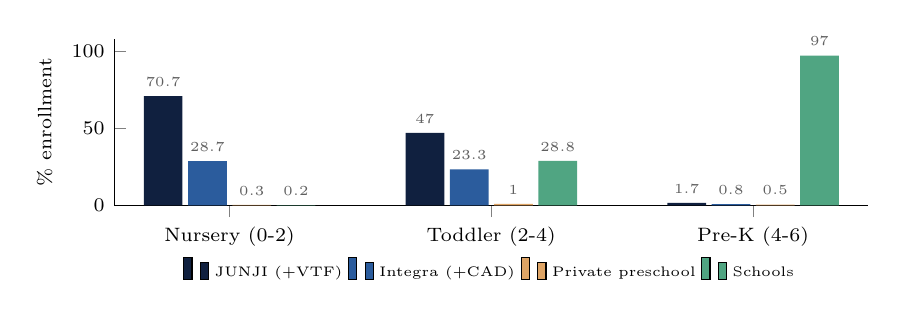
\begin{tikzpicture}
\begin{axis}[
  ybar,
  bar width=14pt,
  width=0.92\textwidth,
  height=3.7cm,
  symbolic x coords={Sala cuna,Nivel medio,Nivel transicion},
  xtick=data,
  xticklabels={Nursery (0-2),Toddler (2-4),Pre-K (4-6)},
  ymin=0, ymax=108,
  ylabel={\% enrollment},
  ylabel style={font=\scriptsize},
  tick label style={font=\scriptsize},
  axis lines*=left,
  enlarge x limits=0.22,
  nodes near coords,
  nodes near coords style={font=\tiny,text=graytext},
  legend style={at={(0.5,-0.27)},anchor=north,legend columns=4,font=\tiny,draw=none},
  grid style={gray!20},
]
\addplot[fill=navy,draw=none] coordinates {(Sala cuna,70.7)(Nivel medio,47.0)(Nivel transicion,1.7)};
\addplot[fill=steel,draw=none] coordinates {(Sala cuna,28.7)(Nivel medio,23.3)(Nivel transicion,0.8)};
\addplot[fill=psuborange,draw=none] coordinates {(Sala cuna,0.3)(Nivel medio,1.0)(Nivel transicion,0.5)};
\addplot[fill=schoolgreen,draw=none] coordinates {(Sala cuna,0.2)(Nivel medio,28.8)(Nivel transicion,97.0)};
\legend{JUNJI (+VTF), Integra (+CAD), Private preschool, Schools}
\end{axis}
\end{tikzpicture}
\end{center}
\vspace{-12pt}
\fuente{Source: authors' elaboration based on Figura 5, Matr\'icula Oficial 2023, Centro de Estudios MINEDUC.}
\takeaway{Ages 0--4: JUNJI and Integra are the main providers --- our focus.}
\end{frame}

% =============================================================================
% 4. IDENTIFICATION DESIGN
% =============================================================================
\begin{frame}{Identification: staggered-adoption event study}
\begin{columns}[T]
\begin{column}{0.66\textwidth}
\begin{itemize}
  \small
  \item \textbf{Design}: staggered-adoption difference-in-differences with event study
  \item \textbf{Unit of treatment}: the UV, the year it opens its first public preschool
  \item \textbf{Unit of analysis}: \textbf{UV $\times$ year} panel, built from a woman $\times$ year panel linked to each woman's UV of residence
  \item \textbf{Fixed effects}: \textbf{UV + year} (baseline); woman FE on the woman $\times$ year panel as a \textbf{robustness check}
  \item \textbf{Estimand}: ATT of UV-level treatment (Baker et al., \emph{JEL} 2026) --- an \textbf{intent-to-treat effect of access}, not individual take-up
\end{itemize}
\end{column}
\begin{column}{0.32\textwidth}
\centering
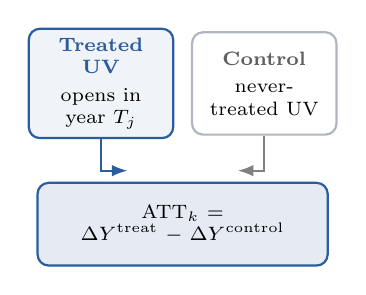
\begin{tikzpicture}[font=\scriptsize]
\node[draw=steel,thick,fill=bgpanel,rounded corners,text width=1.6cm,align=center,minimum height=1.3cm] (a) {\textbf{\textcolor{steel}{Treated UV}}\\[2pt]opens in year $T_j$};
\node[draw=neutralgray,thick,fill=white,rounded corners,text width=1.6cm,align=center,minimum height=1.3cm,right=6pt of a] (b) {\textbf{\textcolor{graytext}{Control}}\\[2pt]never-treated UV};
\coordinate (mid) at ($(a.south)!0.5!(b.south)$);
\node[draw=steel,thick,fill=steel!12,rounded corners,text width=3.45cm,align=center,minimum height=1.05cm,below=16pt of mid] (c) {ATT$_k$ = $\Delta Y^{\text{treat}} - \Delta Y^{\text{control}}$};
\draw[-{Latex[length=2mm]},steel,thick] (a.south) |- ($(c.north)+(-0.7,4pt)$);
\draw[-{Latex[length=2mm]},gray,thick] (b.south) |- ($(c.north)+(0.7,4pt)$);
\end{tikzpicture}
\end{column}
\end{columns}
\takeaway{We compare changes in UVs that get their first preschool vs.\ UVs that never do --- an intent-to-treat effect of access.}
\end{frame}

% =============================================================================
% 5. TREATMENT DEFINITION AND GROUPS
% =============================================================================
\begin{frame}{A UV is treated when it opens its first preschool}
\begin{block}{Treatment definition}
\small A UV is \textbf{treated} the year it opens its first public preschool (JUNJI/Integra) --- goes from 0 to 1+ centers.
\end{block}

\vspace{8pt}
\begin{center}
\small
\begin{tabular}{@{}lp{6.4cm}rr@{}}
\toprule
\textbf{Group} & \textbf{Definition} & \textbf{N (UVs)} & \textbf{\%} \\
\midrule
Excluded        & Already had 1+ center in 2014 (out of design)      & 2{,}265 & 33.0\% \\
Never-treated   & 0 in 2014, stays at 0 through 2024                 & 4{,}145 & 60.5\% \\
Treated         & 0 in 2014, opens first center 2015--2024           & 447     & 6.5\%  \\
\midrule
\textbf{Total universe} & & \textbf{6{,}857} & 100\% \\
\end{tabular}
\end{center}
\fuente{Source: \texttt{base\_cobertura\_cp.dta}. Design sample (\texttt{muestra\_t1==1}) = Never-treated + Treated = 4{,}592 UVs.}
\takeaway{We identify the effect of the first preschool (0 $\to$ 1): 447 treated vs.\ 4{,}145 never-treated.}
\end{frame}

% =============================================================================
% 6. TREATMENT COHORTS BY YEAR
% =============================================================================
\begin{frame}{Treatment cohorts by year}
\begin{columns}[T]
\begin{column}{0.56\textwidth}
\centering
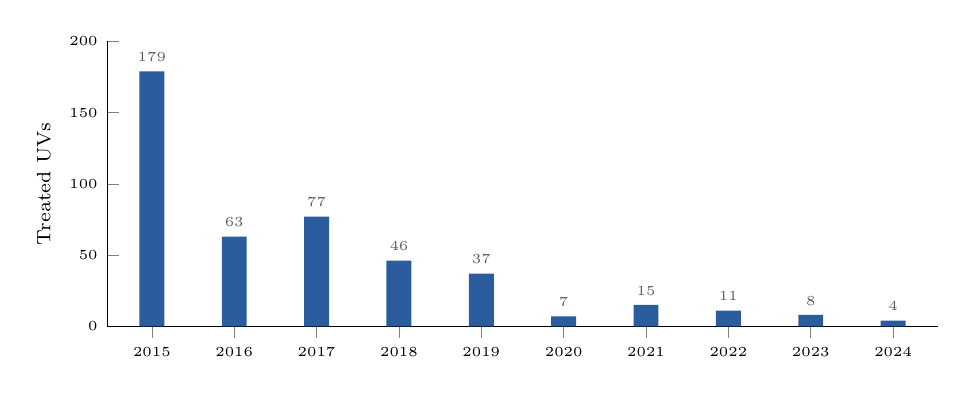
\begin{tikzpicture}
\begin{axis}[
  ybar,
  bar width=9pt,
  width=\linewidth,
  height=5.2cm,
  symbolic x coords={2015,2016,2017,2018,2019,2020,2021,2022,2023,2024},
  xtick=data,
  ymin=0, ymax=200,
  ylabel={Treated UVs},
  ylabel style={font=\scriptsize},
  tick label style={font=\tiny},
  axis lines*=left,
  enlarge x limits=0.06,
  nodes near coords,
  nodes near coords style={font=\tiny,text=graytext},
]
\addplot[fill=steel,draw=none] coordinates {(2015,179)(2016,63)(2017,77)(2018,46)(2019,37)(2020,7)(2021,15)(2022,11)(2023,8)(2024,4)};
\end{axis}
\end{tikzpicture}
\end{column}
\begin{column}{0.42\textwidth}
\begin{itemize}
  \footnotesize
  \item \textbf{2015 cohort is the largest}: 179 UVs (40\%), tied to the Bachelet preschool expansion
  \item \textbf{71\% open in 2015--2017}; only 45 UVs open after 2019
  \item \textbf{2014 as base year} lets us identify the 2015 cohort as 0 $\to$ 1; without it, treated UVs drop from 447 to $\sim$268
\end{itemize}
\end{column}
\end{columns}
\fuente{Source: \texttt{base\_cobertura\_cp.dta}. 447 treated UVs (0 centers in 2014).}
\takeaway{Most openings are early (2015--17): long post-treatment windows for most treated UVs.}
\end{frame}

% =============================================================================
% 7. EMPIRICAL SPECIFICATION AND ESTIMATOR
% =============================================================================
\begin{frame}{Empirical specification and estimator}
\[
Y_{ut} = \lambda_u + \lambda_t + \gamma\,\overline{\text{Age}}_{ut} + \sum_{k \neq -1} \beta_k \, \mathbf{1}\{t - G_u = k\} + \varepsilon_{ut}
\]

\vspace{2pt}
\begin{itemize}
  \footnotesize
  \item $Y_{ut}$: average outcome of women in UV $u$, year $t$ (built from the woman $\times$ year panel). $\lambda_u,\lambda_t$: UV and year fixed effects; SE clustered by UV.
  \item $\overline{\text{Age}}_{ut}$: average age of mothers in the UV-year (labor market specification).
  \item $\beta_k$: effect $k$ years from opening, relative to $k=-1$ (omitted); $k \le -5$ binned.
\end{itemize}

\vspace{4pt}
\begin{block}{Estimation strategy}
\footnotesize \textbf{Baseline TWFE} as reference --- but with staggered treatment, TWFE can use already-treated units as controls (Goodman-Bacon problem). Robust estimator: \textbf{Sun--Abraham} (\texttt{eventstudyinteract}), never-treated UVs as control group. Framework: Baker, Callaway, Cunningham, Goodman-Bacon \& Sant'Anna (\emph{JEL}, 2026).
\end{block}

\vspace{4pt}
\footnotesize \textbf{Main threat}: non-random placement of openings (JUNJI/Integra prioritizing UVs by care demand or socioeconomic profile). \textbf{UV FE} absorb permanent differences across UVs; \textbf{pre-period coefficients} ($k<-1$) test whether trends were already diverging.

\takeaway{Main estimator: Sun--Abraham with never-treated UVs as controls; TWFE as reference.}
\end{frame}

% =============================================================================
% 8. DATA SOURCES AND KEY VARIABLES PER SAMPLE
% =============================================================================
\begin{frame}{Data: what we have and how each sample is built}
\small
\begin{center}
\renewcommand{\arraystretch}{1.35}
\begin{tabular}{@{}>{\raggedright\arraybackslash}p{2.8cm}>{\raggedright\arraybackslash}p{5.0cm}>{\raggedright\arraybackslash}p{4.6cm}@{}}
\toprule
\textbf{Sample} & \textbf{Source data} & \textbf{Key variables} \\
\midrule
Coverage (UV $\times$ year) & JUNJI/Integra transparency requests + UV shapefile (MDSF) & Number of centers, treatment status, opening cohort \\
Women panel (base) & RSH (2016--2024) + FPS (2014--2015) & UV of residence, UV population, child density \\
Labor market & + Rentas (SII/AFC) + Cotizaciones (AFP) & Annual income, months worked, employment \\
Fertility & + Civil Registry birth records (via RIS) & Birth in the year, children under 5 \\
First stage (enrollment) & + Matr\'icula parvularia (child-level) & Enrollment, enrollment rate \\
\bottomrule
\end{tabular}
\end{center}
\takeaway{All administrative registries, linked at the individual level --- no survey self-reports.}
\end{frame}

% =============================================================================
% 9. DATA PIPELINE
% =============================================================================
\begin{frame}{Every preschool is matched to its 2024 neighborhood unit}
\begin{columns}[T]
\begin{column}{0.38\textwidth}
\begin{itemize}
  \footnotesize
  \item Each JUNJI/Integra preschool is \textbf{geolocated} and matched to the UV where it sits (spatial join)
  \item UV boundaries \textbf{changed a lot} over time $\to$ we traced them and mapped everything to \textbf{2024 boundaries}
  \item Preschools and women's UV of residence share \textbf{one common geography} across all years
\end{itemize}
\end{column}
\begin{column}{0.60\textwidth}
\centering
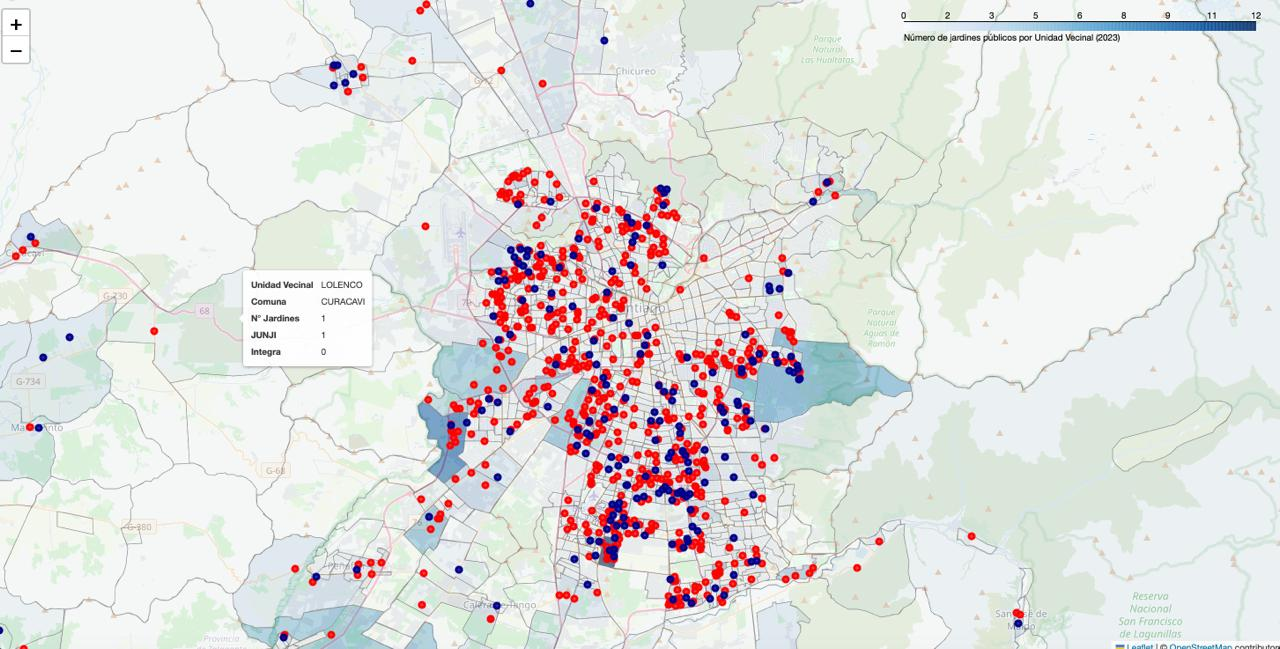
\includegraphics[width=\linewidth,height=0.62\textheight,keepaspectratio]{../jardines_uv_RM.jpeg}
\end{column}
\end{columns}
\fuente{Regi\'on Metropolitana. \textcolor{red}{$\bullet$} JUNJI \quad \textcolor{blue!60!black}{$\bullet$} Integra \quad Shading: public preschools per UV. Source: \texttt{base\_cobertura\_cp.dta}.}
\takeaway{One common geography: every preschool and every woman mapped to 2024 UV boundaries.}
\end{frame}

% =============================================================================
% 9b. MAPS: TREATED UVs
% =============================================================================
\begin{frame}
\vspace{2pt}
\begin{columns}[T]
\begin{column}{0.5\textwidth}
\centering
{\small\textbf{\textcolor{navy}{Regi\'on Metropolitana}}}\\[2pt]
\includegraphics[width=0.98\textwidth,height=0.82\textheight,keepaspectratio]{../output/figures/mapa_uv_tratadas_panel.png}
\end{column}
\begin{column}{0.5\textwidth}
\centering
{\small\textbf{\textcolor{navy}{Valpara\'iso}}}\\[2pt]
\includegraphics[width=0.98\textwidth,height=0.82\textheight,keepaspectratio]{../output/figures/mapa_uv_tratadas_valparaiso.png}
\end{column}
\end{columns}
\fuente{Illustrative examples. Shaded: treated UVs (0 $\to$ 1+ preschools), 2015--2024.}
\end{frame}

% =============================================================================
% 10. WHO IS IN EACH SAMPLE AND WHAT WE MEASURE
% =============================================================================
\begin{frame}{Who is in each sample, and what we measure}
\begin{columns}[T]
\begin{column}{0.48\textwidth}
{\small\textcolor{steel}{\textbf{1. Samples}} \textcolor{graytext}{(selected at the individual level)}}
\begin{itemize}
  \small
  \item \textbf{Fertility}: women of fertile age (18--49)
  \item \textbf{Labor market}: women with a child $<$5 \emph{that specific year} --- not ``ever had a child''
  \item \textbf{First stage}: children of treatment-sample mothers, birth to birth+4
\end{itemize}
\end{column}
\begin{column}{0.48\textwidth}
{\small\textcolor{steel}{\textbf{2. Outcomes}} \textcolor{graytext}{(averaged at UV $\times$ year)}}
\begin{itemize}
  \small
  \item \textbf{Fertility}: share of women who had a child that year (Civil Registry birth records)
  \item \textbf{Labor market}: average annual income, months worked, share employed, dependent vs.\ independent
  \item \textbf{First stage}: enrollment rate
\end{itemize}
\end{column}
\end{columns}

\vspace{8pt}

\takeaway{Each outcome is measured on its relevant population, from administrative records, averaged at the UV $\times$ year level.}
\end{frame}

% =============================================================================
% 11. BALANCE EVIDENCE
% =============================================================================
\begin{frame}{Treated and never-treated UVs look alike --- except in size}
\noindent{\small\textcolor{steel}{\textbf{Labor market sample}} \textcolor{graytext}{(mothers with a child $<$5) --- covariate levels in 2014, before any opening}}\par
\vspace{2pt}
\begin{center}
\scriptsize
\renewcommand{\arraystretch}{0.95}
\setlength{\tabcolsep}{5pt}
\begin{tabular}{@{}lrrrrrrc@{}}
\toprule
 & \multicolumn{3}{c}{Unweighted} & \multicolumn{3}{c}{Weighted by UV population} & \\
\cmidrule(lr){2-4} \cmidrule(lr){5-7}
Variable & Never-tr. & Treated & Norm.\ diff. & Never-tr. & Treated & Norm.\ diff. & Sig.\textsuperscript{a} \\
\midrule
Annual income (M CLP) & 3.60 & 3.55 & -0.033 & 3.95 & 3.89 & -0.039 & * \\
Months worked         & 8.14 & 8.10 & -0.024 & 8.44 & 8.37 & -0.058 & * \\
Age                   & 29.24 & 29.25 & 0.008 & 29.26 & 29.29 & 0.026 & \\
N.\ children $<$5     & 1.11 & 1.11 & 0.045 & 1.11 & 1.11 & 0.049 & \\
Hours worked          & 37.07 & 37.68 & 0.099 & 36.55 & 36.81 & 0.068 & \\
Works (share)         & 0.45 & 0.45 & 0.023 & 0.48 & 0.48 & -0.006 & \\
Education (code)      & 4.98 & 5.02 & 0.028 & 5.20 & 5.18 & -0.020 & \\
\textbf{UV population} & 1126.79 & 2011.08 & \textbf{0.410} & 3530.92 & 5287.26 & \textbf{0.340} & *** \\
Child density 0--5 UV & 0.06 & 0.06 & 0.155 & 0.06 & 0.06 & 0.139 & *** \\
\midrule
N (UVs) & \multicolumn{2}{c}{3{,}909 \ / \ 422} & & \multicolumn{2}{c}{3{,}909 \ / \ 422} & & \\
\bottomrule
\end{tabular}
\end{center}
\vspace{-6pt}
{\tiny \textsuperscript{a} t-test at the woman level (* p$<$0.05, *** p$<$0.01), for reference only; normalized differences prioritized (concern threshold: 0.25).}

\vspace{4pt}
{\footnotesize The UV population gap is \textbf{expected}: the State prioritizes new preschools where need and population are larger. Same pattern in the fertility sample (App.\ A7).}
\takeaway{Selection is in \emph{where} preschools open (UV size), not in \emph{who} lives there $\to$ UV fixed effects.}
\end{frame}

% =============================================================================
% 12. FIRST STAGE -- EVENT STUDY
% =============================================================================
\begin{frame}{Enrollment rises the year a preschool opens and stays higher}
\begin{columns}[c]
\begin{column}{0.62\textwidth}
\centering
{\scriptsize\textbf{Sun--Abraham event study: enrollment rate (weighted)}}\\[1pt]
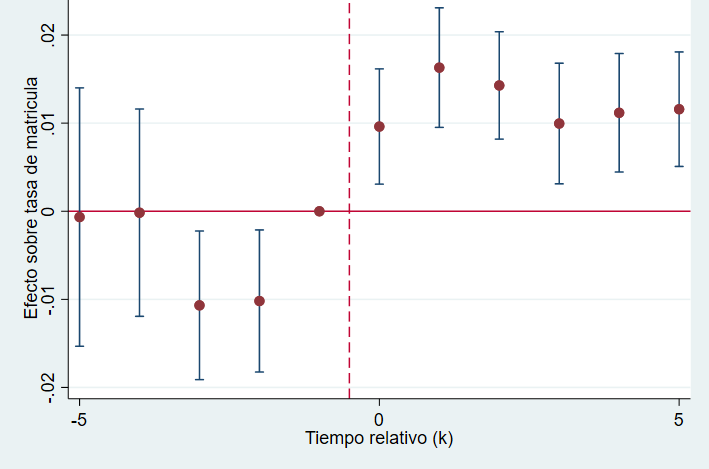
\includegraphics[width=\linewidth,height=0.64\textheight,keepaspectratio]{eventstudy_primera_etapa_sintitulo.png}
\end{column}
\begin{column}{0.36\textwidth}
\colorbox{bgpanel}{\parbox{0.92\linewidth}{\raggedright\footnotesize
Opening a preschool raises the enrollment rate of children aged 0--4 by \textbf{$\approx$1pp} vs.\ never-treated UVs, on a base of $\sim$33\%.

\vspace{4pt}
The effect appears in the \textbf{opening year} and persists for \textbf{at least five years}.}}
\end{column}
\end{columns}
\fuente{Sun--Abraham, weighted by number of children, never-treated UVs as controls, UV and year FE, 95\% CI clustered by UV. Reference $k=-1$.}
\end{frame}

% =============================================================================
% 13. FIRST STAGE -- ROBUSTNESS TABLE
% =============================================================================
\begin{frame}{The enrollment effect is robust across three estimators}
\small
\begin{center}
\begin{tabular}{@{}crrr@{}}
\toprule
{$k$} & {Unweighted TWFE} & {Weighted TWFE} & {Sun--Abraham (unweighted)} \\
\midrule
-5 & -0.002 & -0.015 & 0.006 \\
-4 & -0.009 & -0.011* & 0.004 \\
-3 & -0.013\textsuperscript{\dag} & -0.018*** & -0.005 \\
\textbf{-2} & \textbf{-0.023***} & \textbf{-0.017***} & \textbf{-0.017***} \\
0 & 0.020*** & 0.007* & 0.023*** \\
1 & 0.023*** & 0.013*** & 0.026*** \\
2 & 0.016*** & 0.012*** & 0.019*** \\
3 & 0.018*** & 0.007** & 0.021*** \\
4 & 0.017*** & 0.009** & 0.020*** \\
5 & 0.019*** & 0.009*** & 0.023*** \\
\bottomrule
\end{tabular}
\end{center}
\vspace{4pt}
\footnotesize *** p$<$0.01, ** p$<$0.05, * p$<$0.1, \textsuperscript{\dag} p=0.066. Base rate $\approx$32.6\%. $N=$48,348 UV-year, clusters = 4,568 UVs.

\vspace{6pt}
\normalsize \textbf{Effect: $\approx$2pp on a $\approx$33\% base ($\approx$6\% relative), robust across specifications and growing slightly over time.}
\fuente{Source: \texttt{primera\_etapa.txt}.}
\end{frame}

% =============================================================================
% 14. HONEST PROBLEM: k=-2
% =============================================================================
\begin{frame}{The honest problem: $k=-2$ does not vanish}
\footnotesize
\begin{itemize}
  \item $k=-2$ is \textbf{negative and significant in all three specifications}, and \textbf{survives Sun--Abraham} --- the estimator designed to remove cross-cohort comparison bias
  \item By contrast, $k=-3$ loses significance under unweighted Sun--Abraham (p=0.066 $\to$ p=0.429)
\end{itemize}

\vspace{5pt}
\begin{block}{Hypotheses under investigation (none confirmed)}
\footnotesize
\begin{itemize}
  \item \textbf{1. Registration lag / construction transition}: the recorded opening year may lag actual full-capacity operation
  \item \textbf{2. Age-cutoff measurement} (\texttt{edad\_30\_06}): possible source of noise, no confirmed mechanical link to $k=-2$ specifically
  \item \textbf{3. Partial COVID overlap}: weak, covers only cohorts with $g1\in[2021,2023]$
\end{itemize}
\end{block}

\end{frame}

% =============================================================================
% 17. NEXT STEPS
% =============================================================================
\begin{frame}{Next steps}
\begin{columns}[T]
\begin{column}{0.33\textwidth}
\begin{block}{Immediate}
\footnotesize
\begin{itemize}
  \item Finish labor market estimation
  \item Finish fertility estimation
\end{itemize}
\end{block}
\end{column}
\begin{column}{0.33\textwidth}
\begin{block}{Short term}
\footnotesize
\begin{itemize}
  \item Disaggregate $k=-2$ by opening cohort
  \item Heterogeneity by education level (nursery/toddler vs.\ pre-K)
\end{itemize}
\end{block}
\end{column}
\begin{column}{0.33\textwidth}
\begin{block}{Medium term}
\footnotesize
\begin{itemize}
  \item Robustness: weighted vs.\ unweighted, outlier UVs
  \item Write results section
\end{itemize}
\end{block}
\end{column}
\end{columns}
\end{frame}

% =============================================================================
% APPENDIX
% =============================================================================
\appendix
\begin{frame}[plain]
\vspace{60pt}
\begin{center}
{\LARGE\bfseries\color{navy} Appendix}
\end{center}
\end{frame}

% -----------------------------------------------------------------------
\begin{frame}{Appendix A1. Enrollment by dependency, 2018--2022}
\begin{center}
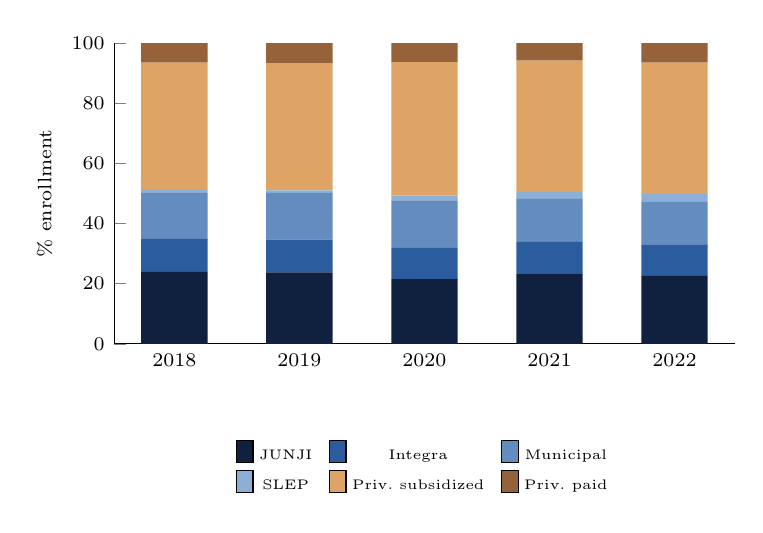
\begin{tikzpicture}
\begin{axis}[
  ybar stacked,
  bar width=24pt,
  width=0.78\textwidth,
  height=5.4cm,
  symbolic x coords={2018,2019,2020,2021,2022},
  xtick=data,
  ymin=0, ymax=100,
  ylabel={\% enrollment},
  ylabel style={font=\scriptsize},
  tick label style={font=\scriptsize},
  axis lines*=left,
  enlarge x limits=0.12,
  legend style={at={(0.5,-0.3)},anchor=north,legend columns=3,font=\tiny,draw=none,/tikz/every even column/.append style={column sep=4pt}},
  grid style={gray!20},
]
\addplot[fill=navy,draw=none] coordinates {(2018,23.94)(2019,23.79)(2020,21.52)(2021,23.16)(2022,22.61)};
\addplot[fill=steel,draw=none] coordinates {(2018,11.14)(2019,10.89)(2020,10.35)(2021,10.70)(2022,10.45)};
\addplot[fill=municblue,draw=none] coordinates {(2018,15.30)(2019,15.54)(2020,15.87)(2021,14.31)(2022,14.34)};
\addplot[fill=steellight,draw=none] coordinates {(2018,0.79)(2019,0.80)(2020,1.53)(2021,2.33)(2022,2.36)};
\addplot[fill=psuborange,draw=none] coordinates {(2018,42.35)(2019,42.32)(2020,44.40)(2021,43.67)(2022,43.78)};
\addplot[fill=ppagbrown,draw=none] coordinates {(2018,6.47)(2019,6.67)(2020,6.35)(2021,5.84)(2022,6.47)};
\legend{JUNJI, Integra, Municipal, SLEP, Priv.\ subsidized, Priv.\ paid}
\end{axis}
\end{tikzpicture}
\end{center}
\fuente{Source: Tabla 14, Matr\'icula Oficial Educaci\'on Parvularia por dependencia 2018--2022, Centro de Estudios MINEDUC.}
\end{frame}

% -----------------------------------------------------------------------
\begin{frame}{Appendix A2. Full identification assumptions and placebo check}
\begin{itemize}
  \item \textbf{Parallel trends}: assessed via pre-opening event-study coefficients; should be statistically indistinguishable from zero
  \item \textbf{No anticipation}: mothers do not adjust decisions before the effective opening --- depends on how much advance notice openings receive (to analyze)
  \item \textbf{Exogeneity of timing}: opening timing should not correlate with unobserved UV characteristics. \textbf{Main threat}: JUNJI/Integra may prioritize UVs with higher care demand or specific socioeconomic profiles
\end{itemize}

\vspace{10pt}
\begin{block}{Placebo check}
\small An analogous event study will be estimated using the \textbf{pre-treatment birth rate} of the UV as the outcome. Non-significant pre-treatment coefficients would strengthen the parallel-trends assumption of the main model.
\end{block}
\end{frame}

% -----------------------------------------------------------------------
\begin{frame}{Appendix A3. Weighted vs.\ unweighted robustness}
\begin{itemize}
  \item Weighted specification (by \texttt{n\_ninos}) shows a visibly worse pre-trend: 3 of 4 pre-period coefficients significant, vs.\ 1 of 4 unweighted
  \item Consistent with a small number of large outlier UVs dominating the weighted average: \texttt{n\_ninos} median 40, mean 78, p99 541, max $\approx$3{,}200
  \item \textbf{Pending}: robustness check excluding or capping the largest UVs
\end{itemize}
\end{frame}

% -----------------------------------------------------------------------
\begin{frame}{Appendix A4. Data limitation: UV assignment in 2014--2015}
\begin{itemize}
  \item FPS (2014--2015) has no reliable UV field $\to$ those two years are anchored to the woman's \textbf{2016 UV} as a proxy
  \item \textbf{Consequence}: women who left the panel before 2016 are dropped from 2014--2015 --- precisely the earliest pre-trend years
  \item RIS has not delivered a better historical crosswalk despite repeated requests; only unstandardized UV name strings are available
  \item \textbf{Idea, not yet tested}: fuzzy matching on UV name strings
\end{itemize}
\end{frame}

% -----------------------------------------------------------------------
\begin{frame}{Appendix A5. Panel composition over time}
\vspace{-10pt}
\begin{center}
{\rmfamily
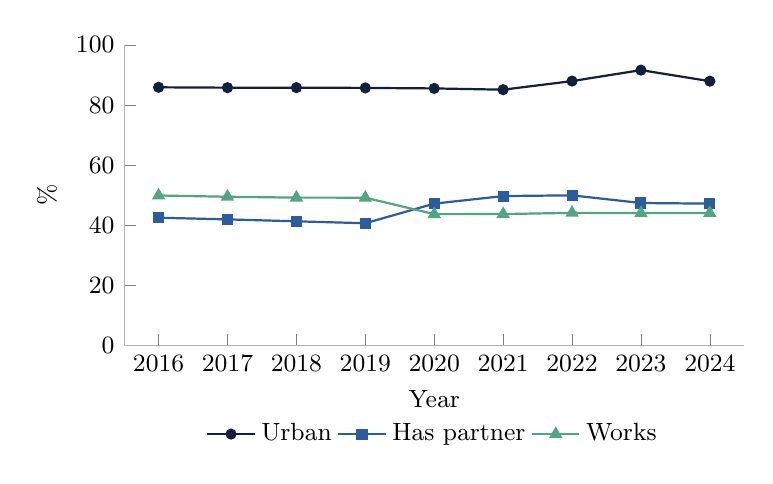
\begin{tikzpicture}
\begin{axis}[
  width=0.78\textwidth,
  height=5.4cm,
  xmin=2015.5, xmax=2024.5,
  ymin=0, ymax=100,
  xtick={2016,2017,2018,2019,2020,2021,2022,2023,2024},
  ytick={0,20,40,60,80,100},
  xlabel={Year},
  ylabel={\%},
  xlabel style={font=\small},
  ylabel style={font=\small},
  tick label style={font=\small},
  scaled x ticks=false,
  /pgf/number format/1000 sep=,
  axis lines*=left,
  axis line style={gray!60},
  legend style={at={(0.5,-0.22)},anchor=north,legend columns=3,font=\small,draw=none},
  legend cell align=left,
]
\addplot[navy,mark=*,mark size=1.6pt,thick] coordinates {
  (2016,85.90)(2017,85.78)(2018,85.79)(2019,85.70)(2020,85.53)(2021,85.11)(2022,87.97)(2023,91.62)(2024,87.94)
};
\addplot[steel,mark=square*,mark size=1.6pt,thick] coordinates {
  (2016,42.53)(2017,41.97)(2018,41.33)(2019,40.69)(2020,47.21)(2021,49.73)(2022,49.97)(2023,47.42)(2024,47.21)
};
\addplot[schoolgreen,mark=triangle*,mark size=2pt,thick] coordinates {
  (2016,49.92)(2017,49.50)(2018,49.21)(2019,49.20)(2020,43.72)(2021,43.74)(2022,44.15)(2023,44.07)(2024,44.09)
};
\legend{Urban, Has partner, Works}
\end{axis}
\end{tikzpicture}
}
\end{center}
\fuente{Panel of women aged 18--70 (RSH), 2016--2024.}
\end{frame}

% -----------------------------------------------------------------------
\begin{frame}{Appendix A6. Task status}
\vspace{-8pt}
\tiny
\setlength{\tabcolsep}{2.5pt}
\renewcommand{\arraystretch}{0.85}
\begin{center}
\begin{tabular}{@{}p{1.3cm}p{4.0cm}c p{6.0cm}@{}}
\toprule
\textbf{Block} & \textbf{Task} & \textbf{Status} & \textbf{Note} \\
\midrule
\multirow{6}{1.3cm}{\shortstack[l]{2. Data\\generation}}
 & Coverage base (preschools $\times$ UV, 2014--2024) & {\color{statuslisto}\textbf{ready}} & Verified; private preschools (transparency) still a possible extension \\
 & Women panel (2014--2024, incl.\ FPS anchor) & {\color{statuslisto}\textbf{ready}} & 2014--2015 anchored to 2016 UV (see A5) \\
 & Rentas / Cotizaciones cleaning & {\color{schoolgreen}\textbf{advanced}} & Independent/state/FF.AA.\ cotizaciones still pending \\
 & Children registry cleaning & {\color{statuslisto}\textbf{ready}} & \texttt{tuvo\_hijo}, \texttt{n\_hijos\_menor5} \\
 & Merge panel + outcome variables & {\color{statuslisto}\textbf{ready}} & By \texttt{rut\_inn} \\
 & Treated / non-treated definition & {\color{statuslisto}\textbf{ready}} & \texttt{grupo\_t1}, \texttt{g1}, \texttt{muestra\_t1} \\
\midrule
\multirow{2}{1.3cm}{\shortstack[l]{3. Panel\\analysis}}
 & First-stage estimation (enrollment) & {\color{statuslisto}\textbf{ready}} & 3 specifications; $k=-2$ open issue \\
 & Balance / validity check & {\color{statuslisto}\textbf{ready}} & UV-level balance table \\
\midrule
\multirow{4}{1.3cm}{\shortstack[l]{4. Data\\analysis}}
 & Methodology choice & {\color{statuslisto}\textbf{ready}} & Sun--Abraham within Baker et al.\ (JEL 2026) framework \\
 & Treatment definition & {\color{statuslisto}\textbf{ready}} & Extensive margin, 0$\to$1 \\
 & Run regressions (labor, fertility) & {\color{statuspink}\textbf{in progress}} & Expected before Thursday \\
 & Analyze results & {\color{statuspink}\textbf{in progress}} & First stage analyzed; rest pending \\
\midrule
\multirow{2}{1.3cm}{\shortstack[l]{5. Mechanisms}}
 & Heterogeneity by group / level & {\color{statusred}\textbf{not started}} & \\
 & Public-policy implications & {\color{statusred}\textbf{not started}} & \\
\midrule
\shortstack[l]{6. Writing} & --- & {\color{statuspink}\textbf{in progress}} & \\
\bottomrule
\end{tabular}
\end{center}
\end{frame}

% A7. Balance -- fertility sample
\begin{frame}{Appendix A7. Balance in the fertility sample}
\noindent{\small\textcolor{steel}{\textbf{Fertility sample}} \textcolor{graytext}{(women aged 18--49) --- covariate levels in 2014, before any opening}}\par
\vspace{2pt}
\begin{center}
\scriptsize
\renewcommand{\arraystretch}{0.95}
\setlength{\tabcolsep}{5pt}
\begin{tabular}{@{}lrrrrrrc@{}}
\toprule
 & \multicolumn{3}{c}{Unweighted} & \multicolumn{3}{c}{Weighted by UV population} & \\
\cmidrule(lr){2-4} \cmidrule(lr){5-7}
Variable & Never-tr. & Treated & Norm.\ diff. & Never-tr. & Treated & Norm.\ diff. & Sig.\textsuperscript{a} \\
\midrule
Birth rate            & 0.057 & 0.058 & 0.031 & 0.06 & 0.060 & 0.051 & \\
Age                   & 31.90 & 31.83 & -0.053 & 31.74 & 31.82 & 0.095 & \\
Children $<$5 per woman & 0.303 & 0.319 & 0.156 & 0.31 & 0.320 & 0.117 & ** \\
\textbf{UV population} & 1111.42 & 2025.96 & \textbf{0.423} & 3540.63 & 5305.76 & \textbf{0.342} & *** \\
Child density 0--5 UV & 0.0590 & 0.0631 & 0.176 & 0.06 & 0.064 & 0.148 & ** \\
\textbf{Women in sample per UV} & 233.60 & 445.45 & \textbf{0.401} & 795.29 & 1234.46 & \textbf{0.347} & *** \\
\midrule
N (UVs) & \multicolumn{2}{c}{3{,}973 \ / \ 422} & & \multicolumn{2}{c}{3{,}973 \ / \ 422} & & \\
\bottomrule
\end{tabular}
\end{center}
\vspace{-6pt}
{\tiny \textsuperscript{a} t-test at the UV level (** p$<$0.01, *** p$<$0.001), for reference only; normalized differences prioritized (concern threshold: 0.25). UVs with at least one sample woman in 2014, hence more never-treated UVs than in the labor sample.}
\takeaway{Same conclusion as the labor sample: women look alike, UVs differ in size.}
\end{frame}

\end{document}
